% ============================================================
% IEEE TDSC Paper — LaTeX Source (Expanded for 8–10 pages)
% "A Semantic Security Layer for ONNX-Deployed Network
%  Intrusion Detection at the Edge"
% ============================================================
\documentclass[journal]{IEEEtran}

% ── Packages ──
\usepackage{amsmath,amssymb,amsfonts}
\usepackage{graphicx}
\usepackage{textcomp}
\usepackage{xcolor}
\usepackage{cite}
\usepackage{booktabs}
\usepackage{multirow}
\usepackage{url}
\usepackage{hyperref}
\usepackage{algorithm}
\usepackage{algorithmic}
\usepackage{balance}
\usepackage{enumitem}
\usepackage{subcaption}

% ── Macro shortcuts ──
\newcommand{\ie}{\emph{i.e.}}
\newcommand{\eg}{\emph{e.g.}}
\newcommand{\cf}{\emph{cf.}}
\newcommand{\etal}{\emph{et~al.}}
\newcommand{\sysname}{\textsc{SemanticShield}}

% ============================================================
\begin{document}

\title{A Semantic Security Layer for ONNX-Deployed Network Intrusion Detection at the Edge}

% AUTHOR BLOCK — update with your supervisor info
\author{Muhammad~Sikandar~Hussain%
  \thanks{M.~S.~Hussain is with CNIT/PNTLab Pisa, TECIP Institute, Scuola Superiore Sant'Anna, Pisa, Italy (e-mail: m.hussain@santannapisa.it).}%
  % Add supervisor(s) here:
  % \and Supervisor~Name%
  % \thanks{S.~Name is with Department, Institution, City, Country.}%
}

\markboth{IEEE Transactions on Dependable and Secure Computing, Vol.~XX, No.~XX, 2026}%
{Hussain: A Semantic Security Layer for ONNX-Deployed NIDS}

\maketitle

% ============================================================
% ABSTRACT
% ============================================================
\begin{abstract}
Machine-learning-based network intrusion detection systems (ML-NIDS) are increasingly deployed on resource-constrained edge gateways using the ONNX Runtime inference engine. However, once a model is exported to ONNX and deployed, no standard mechanism exists to detect distribution drift, validate input integrity, or flag unreliable predictions at inference time---the very moment when silent failures have operational consequences. We present \sysname{}, a \emph{semantic security layer} that augments ONNX-deployed NIDS classifiers with three runtime monitors operating on the deployed computational graph itself: (i)~a confidence analyzer using Maximum Softmax Probability (MSP) thresholding, (ii)~a distribution drift detector that extracts intermediate-layer embeddings from a dual-output ONNX export and evaluates class-conditional Mahalanobis and angular distances, and (iii)~an input validator that catches schema mismatches, zero-fill corruption, and statistical outliers. Our evaluation on CSE-CIC-IDS2018 and NF-ToN-IoT-v2 with five-seed statistical rigor demonstrates that the multi-signal composite engine achieves an out-of-distribution AUROC of 0.966 (surpassing both Mahalanobis at 0.959 and MSP at 0.850) and intercepts 100\% of noise inputs and 100\% of zero-filled inputs while adding only 0.29\,ms overhead to a 0.06\,ms baseline (0.35\,ms total per flow). We further report a \emph{negative result}: standardizing features to NetFlow format eliminates zero-filling but does not rescue cross-dataset generalization (multi-class F1 collapses from 0.77 to 0.06), and a per-field semantic audit reveals that 38\% of supposedly matched features measure physically different quantities. A multi-precision quantization study shows FP16 achieves zero-cost 50\% compression, static INT8 causes catastrophic accuracy loss ($-$38\% F1), while weight-only INT4 preserves 97.8\% of F1 with 81\% size reduction. All experiments are conducted on the deployed ONNX graph without requiring the original PyTorch model at inference time.
\end{abstract}

\begin{IEEEkeywords}
Network intrusion detection, ONNX Runtime, out-of-distribution detection, edge inference, distribution drift, model quantization, semantic validation
\end{IEEEkeywords}


% ============================================================
% SECTION I — INTRODUCTION
% ============================================================
\section{Introduction}
\label{sec:introduction}

\IEEEPARstart{M}{achine}-learning-based network intrusion detection systems (ML-NIDS) have demonstrated strong classification performance on curated benchmark datasets such as CSE-CIC-IDS2018~\cite{sharafaldin2018cicids} and ToN-IoT~\cite{moustafa2021toniot}, with reported F1 scores frequently exceeding 0.95 in controlled evaluations. The Open Neural Network Exchange (ONNX) format has emerged as the de facto standard for deploying trained models from research frameworks (PyTorch, TensorFlow) onto production inference engines~\cite{onnxruntime2024}. This is particularly relevant for edge gateways---IoT routers, industrial switches, and campus network appliances---where framework-agnostic, low-latency inference is essential for real-time traffic classification.

However, the transition from training to deployment introduces a critical \emph{security gap} that the existing ML-NIDS literature largely overlooks. Once a model is exported to ONNX and shipped to an edge device, \emph{no standard runtime mechanism} verifies that the inference environment matches the assumptions encoded during training. Three classes of failure occur silently in production:

\textbf{Distribution drift.} Network traffic patterns shift seasonally, geographically, and with evolving attack campaigns, causing classifier accuracy to degrade without generating any error signal~\cite{aceto2024driftNIDS}. A model trained on 2018 traffic may encounter novel attack variants, new applications, or fundamentally different traffic mixes, yet continues to produce confident---and incorrect---predictions.

\textbf{Input corruption and schema mismatch.} Feature extractors differ between deployments: CICFlowMeter and nProbe NetFlow produce features with the same names but potentially different physical semantics~\cite{sarhan2022nftoniot}. When features are mapped by name alone, semantically invalid inputs are silently injected into the model, a problem we quantify in Section~\ref{sec:audit}.

\textbf{Adversarial manipulation.} Crafted inputs can exploit model blind spots, a risk amplified when the deployed model lacks any mechanism to flag its own uncertainty~\cite{apruzzese2023adversarialML}. The MITRE ATT\&CK framework~\cite{mitre2024} identifies ML model evasion as a growing threat category.

Recent work has explored out-of-distribution (OOD) detection as a candidate runtime monitoring layer for NIDS~\cite{mclaughlin2023oodforNIDS,netsight2025}. However, existing approaches share two significant limitations. First, they evaluate exclusively on unconstrained server hardware without considering the latency and memory budgets of edge deployment. Second, they require the original training framework (PyTorch or TensorFlow) at inference time to extract intermediate features---defeating the purpose of ONNX-based deployment.

This paper addresses these limitations by presenting \sysname{}, a semantic security layer designed for the specific constraints of ONNX-deployed edge NIDS. Our contributions are:

\begin{enumerate}[leftmargin=*]
  \item \textbf{Dual-output ONNX architecture for sub-millisecond semantic monitoring.} We re-export the trained classifier with an auxiliary output that exposes the penultimate hidden layer (a 64-dimensional embedding), enabling a composite runtime monitor to execute directly on the deployed computational graph. The complete multi-signal analysis pipeline---confidence scoring, class-conditional drift detection, and input validation---achieves AUROC = 0.966 for OOD detection and adds only 0.29\,ms to the 0.06\,ms baseline inference, for a total of 0.35\,ms per flow, well within real-time edge budgets.

  \item \textbf{Empirical semantic schema audit of cross-dataset feature mappings.} We conduct the first per-field physical-quantity reconciliation between CICFlowMeter (76 features) and nProbe NetFlow (21 mapped features), demonstrating that 8 of 21 mapped pairs (38\%) measure fundamentally different physical quantities---\eg, throughput rate (bits/second) mapped to raw header byte count. This finding partially explains the persistent cross-dataset generalization failure reported across the NIDS literature~\cite{pontes2021crossdataset,cantone2024crossdataset} and has implications for any cross-dataset NIDS benchmark.

  \item \textbf{Multi-precision quantization trade-off analysis for edge deployment.} We evaluate FP32, FP16, static INT8, and weight-only INT4 (MatMulNBits) quantization on the same model and dataset, revealing a counterintuitive result: weight-only INT4 (81\% size reduction, $-$2.2\% F1) substantially outperforms static INT8 (73\% size reduction, $-$38\% F1) because static quantization clips intermediate activations whose dynamic range is poorly modeled by calibration.
\end{enumerate}

The remainder of this paper is organized as follows. Section~\ref{sec:related} surveys related work on OOD detection, NIDS generalization, and ONNX deployment security. Section~\ref{sec:method} presents the \sysname{} architecture and its three component analyzers. Section~\ref{sec:audit} details the NetFlow semantic schema audit and the ``cleaning hurts transfer'' negative finding. Section~\ref{sec:evaluation} reports comprehensive experimental results with five-seed statistical rigor. Section~\ref{sec:discussion} discusses embedding geometry, multi-signal ensembling, and quantization dynamics. Section~\ref{sec:conclusion} concludes the paper and outlines future work.


% ============================================================
% SECTION II — RELATED WORK
% ============================================================
\section{Related Work}
\label{sec:related}

\subsection{Out-of-Distribution Detection for Deep Classifiers}

Out-of-distribution detection aims to identify test-time inputs that differ significantly from the training distribution, enabling classifiers to abstain rather than produce unreliable predictions. The foundational work of Hendrycks and Gimpel~\cite{hendrycks2017baseline} established Maximum Softmax Probability (MSP) as a simple yet surprisingly effective baseline: well-classified in-distribution inputs tend to have higher maximum softmax probabilities than OOD inputs. Despite its simplicity, MSP remains competitive with more complex approaches, particularly for networks with well-calibrated output distributions.

Lee~\etal~\cite{lee2018mahalanobis} proposed a principled approach based on the Mahalanobis distance computed over intermediate-layer features, modeling each class's feature distribution as a multivariate Gaussian and computing the log-likelihood of test inputs relative to the closest class centroid under a tied covariance matrix. While effective on computer vision benchmarks, applying Mahalanobis monitoring to network flow embeddings requires careful attention to covariance regularization and per-class clustering to avoid degenerate distance metrics in multimodal intrusion traffic (Section~\ref{sec:discussion}).

Liu~\etal~\cite{liu2020energy} introduced energy-based OOD scoring as a theoretically grounded alternative to MSP, proving that the free energy of the logit vector is aligned with the probability density of inputs. Liang~\etal~\cite{liang2018odin} proposed ODIN, combining temperature scaling with input perturbation to amplify the separation between in-distribution and OOD softmax scores. Sun~\etal~\cite{sun2021react} introduced ReAct, which truncates penultimate-layer activations at a threshold to reduce the overconfidence phenomenon on OOD inputs.

\textbf{Positioning.} Our work leverages MSP, class-conditional Mahalanobis distance, and deterministic schema validation within an integrated edge monitoring layer (Section~\ref{sec:evaluation}). The key distinction is deployment context: existing methods assume access to the training framework. Our implementation operates on a \emph{dual-output ONNX export}---a single forward pass through the deployed graph returns both logits and intermediate embeddings, requiring neither PyTorch nor TensorFlow at inference time.

\subsection{OOD Detection Specifically for Network Intrusion Detection}

The application of OOD detection to NIDS is a nascent but growing research area. McLaughlin and del Rinc\'{o}n~\cite{mclaughlin2023oodforNIDS} conducted the most comprehensive evaluation to date, testing six OOD detection methods (MSP, ODIN, Mahalanobis, Energy, ViM, KNN) as a runtime layer for NIDS classifiers in cross-dataset scenarios. They reported near-100\% detection of shifted traffic on several dataset pairs, though with significant variation across detectors and datasets.

Pratt~\etal~\cite{netsight2025} proposed NetSight for online distribution-shift detection with continuous adaptation via pseudo-labeling and knowledge distillation, demonstrating that adaptive approaches can maintain detection performance as traffic evolves. Their focus is on continuous adaptation rather than deployment-time monitoring.

\textbf{Distinction.} Neither study evaluates under the constraints of edge deployment: quantized models, sub-millisecond latency budgets, and containerized microservice architectures. McLaughlin and del Rinc\'{o}n~\cite{mclaughlin2023oodforNIDS} note that naive Mahalanobis distance can perform inconsistently across NIDS datasets when reference distributions are poorly conditioned. Our work specifically targets the ONNX-exported deployment artifact, incorporates regularized class-conditional Mahalanobis embeddings, and demonstrates feasibility under aggressive quantization (INT4 weight-only) with end-to-end latency profiling from in-memory inference to REST API serving.

\subsection{Cross-Dataset Generalization in NIDS}

Cross-dataset generalization remains a fundamental unsolved challenge in NIDS research. Sarhan~\etal~\cite{sarhan2022nftoniot} proposed NetFlow-based feature standardization across NIDS datasets, creating normalized versions (NF-ToN-IoT-v2, NF-BoT-IoT, NF-CSE-CIC-IDS2018) designed to enable direct model transfer. While this eliminates the zero-filling problem caused by dimension mismatches, it does not address the deeper issue of \emph{semantic equivalence} between feature extractors.

Pontes~\etal~\cite{pontes2021crossdataset} evaluated transferability between CIC-IDS and CTU-13, reporting that binary classification (benign vs.\ attack) achieves F1 $\approx 0.74$, but multi-class attack-type classification collapses to F1 $< 0.10$. Cantone~\etal~\cite{cantone2024crossdataset} systematically demonstrated this degradation across five dataset pairs, attributing the failure to differences in feature extraction pipelines and attack methodology.

\textbf{Contribution.} Our semantic schema audit (Section~\ref{sec:audit}) goes beyond field-name matching to verify \emph{physical-quantity equivalence}, revealing that 38\% of mapped features are semantic mismatches. This provides the first concrete, per-field explanation for the persistent F1 collapse, rather than attributing it to generic ``distribution shift.''

\subsection{ONNX Model Security and Deployment Integrity}

The ONNX ecosystem introduces security concerns at the converter level. Jajal~\etal~\cite{jajal2024onnxfailures} surveyed 92 software engineers and systematically analyzed 200 GitHub issues from ONNX converter repositories, finding that 33\% of reported failures produce semantically incorrect models that pass ONNX validation without any error signal. This represents a supply-chain risk: a model that produces subtly wrong predictions in production, without any mechanism to detect the discrepancy.

Our work addresses a complementary concern: even when the ONNX conversion is faithful, the \emph{deployment environment} may diverge from training assumptions due to input schema changes, distribution drift, or adversarial manipulation. The \sysname{} engine provides runtime monitoring that operates within the ONNX ecosystem, using only ONNX Runtime APIs and NumPy for all computations.


% ============================================================
% SECTION III — PROPOSED METHOD
% ============================================================
\section{Proposed Method: \sysname{}}
\label{sec:method}

\subsection{System Architecture}

Fig.~\ref{fig:architecture} illustrates the \sysname{} architecture. A PyTorch MLP classifier (ThreatMLP: 4 layers with dimensions $d \rightarrow 256 \rightarrow 128 \rightarrow 64 \rightarrow C$, where $d$ is the input feature dimensionality and $C = 15$ attack classes) is re-exported to ONNX with a \emph{dual-output} configuration. The primary output provides the standard classification logits, while an auxiliary output exposes the 64-dimensional penultimate hidden layer embedding (fc3). At inference time, ONNX Runtime executes the full computational graph and returns both outputs in a single forward pass with negligible additional overhead.

The dual-output export is achieved by wrapping the trained model in a lightweight \texttt{ThreatMLPWithEmbedding} wrapper that intercepts the fc3 activation via a forward hook, then exports the combined model using \texttt{torch.onnx.export} with two named outputs (\texttt{logits} and \texttt{embedding}). This approach requires no architectural changes to the original model and preserves all learned parameters exactly.

% Architecture figure
\begin{figure*}[t]
  \centering
  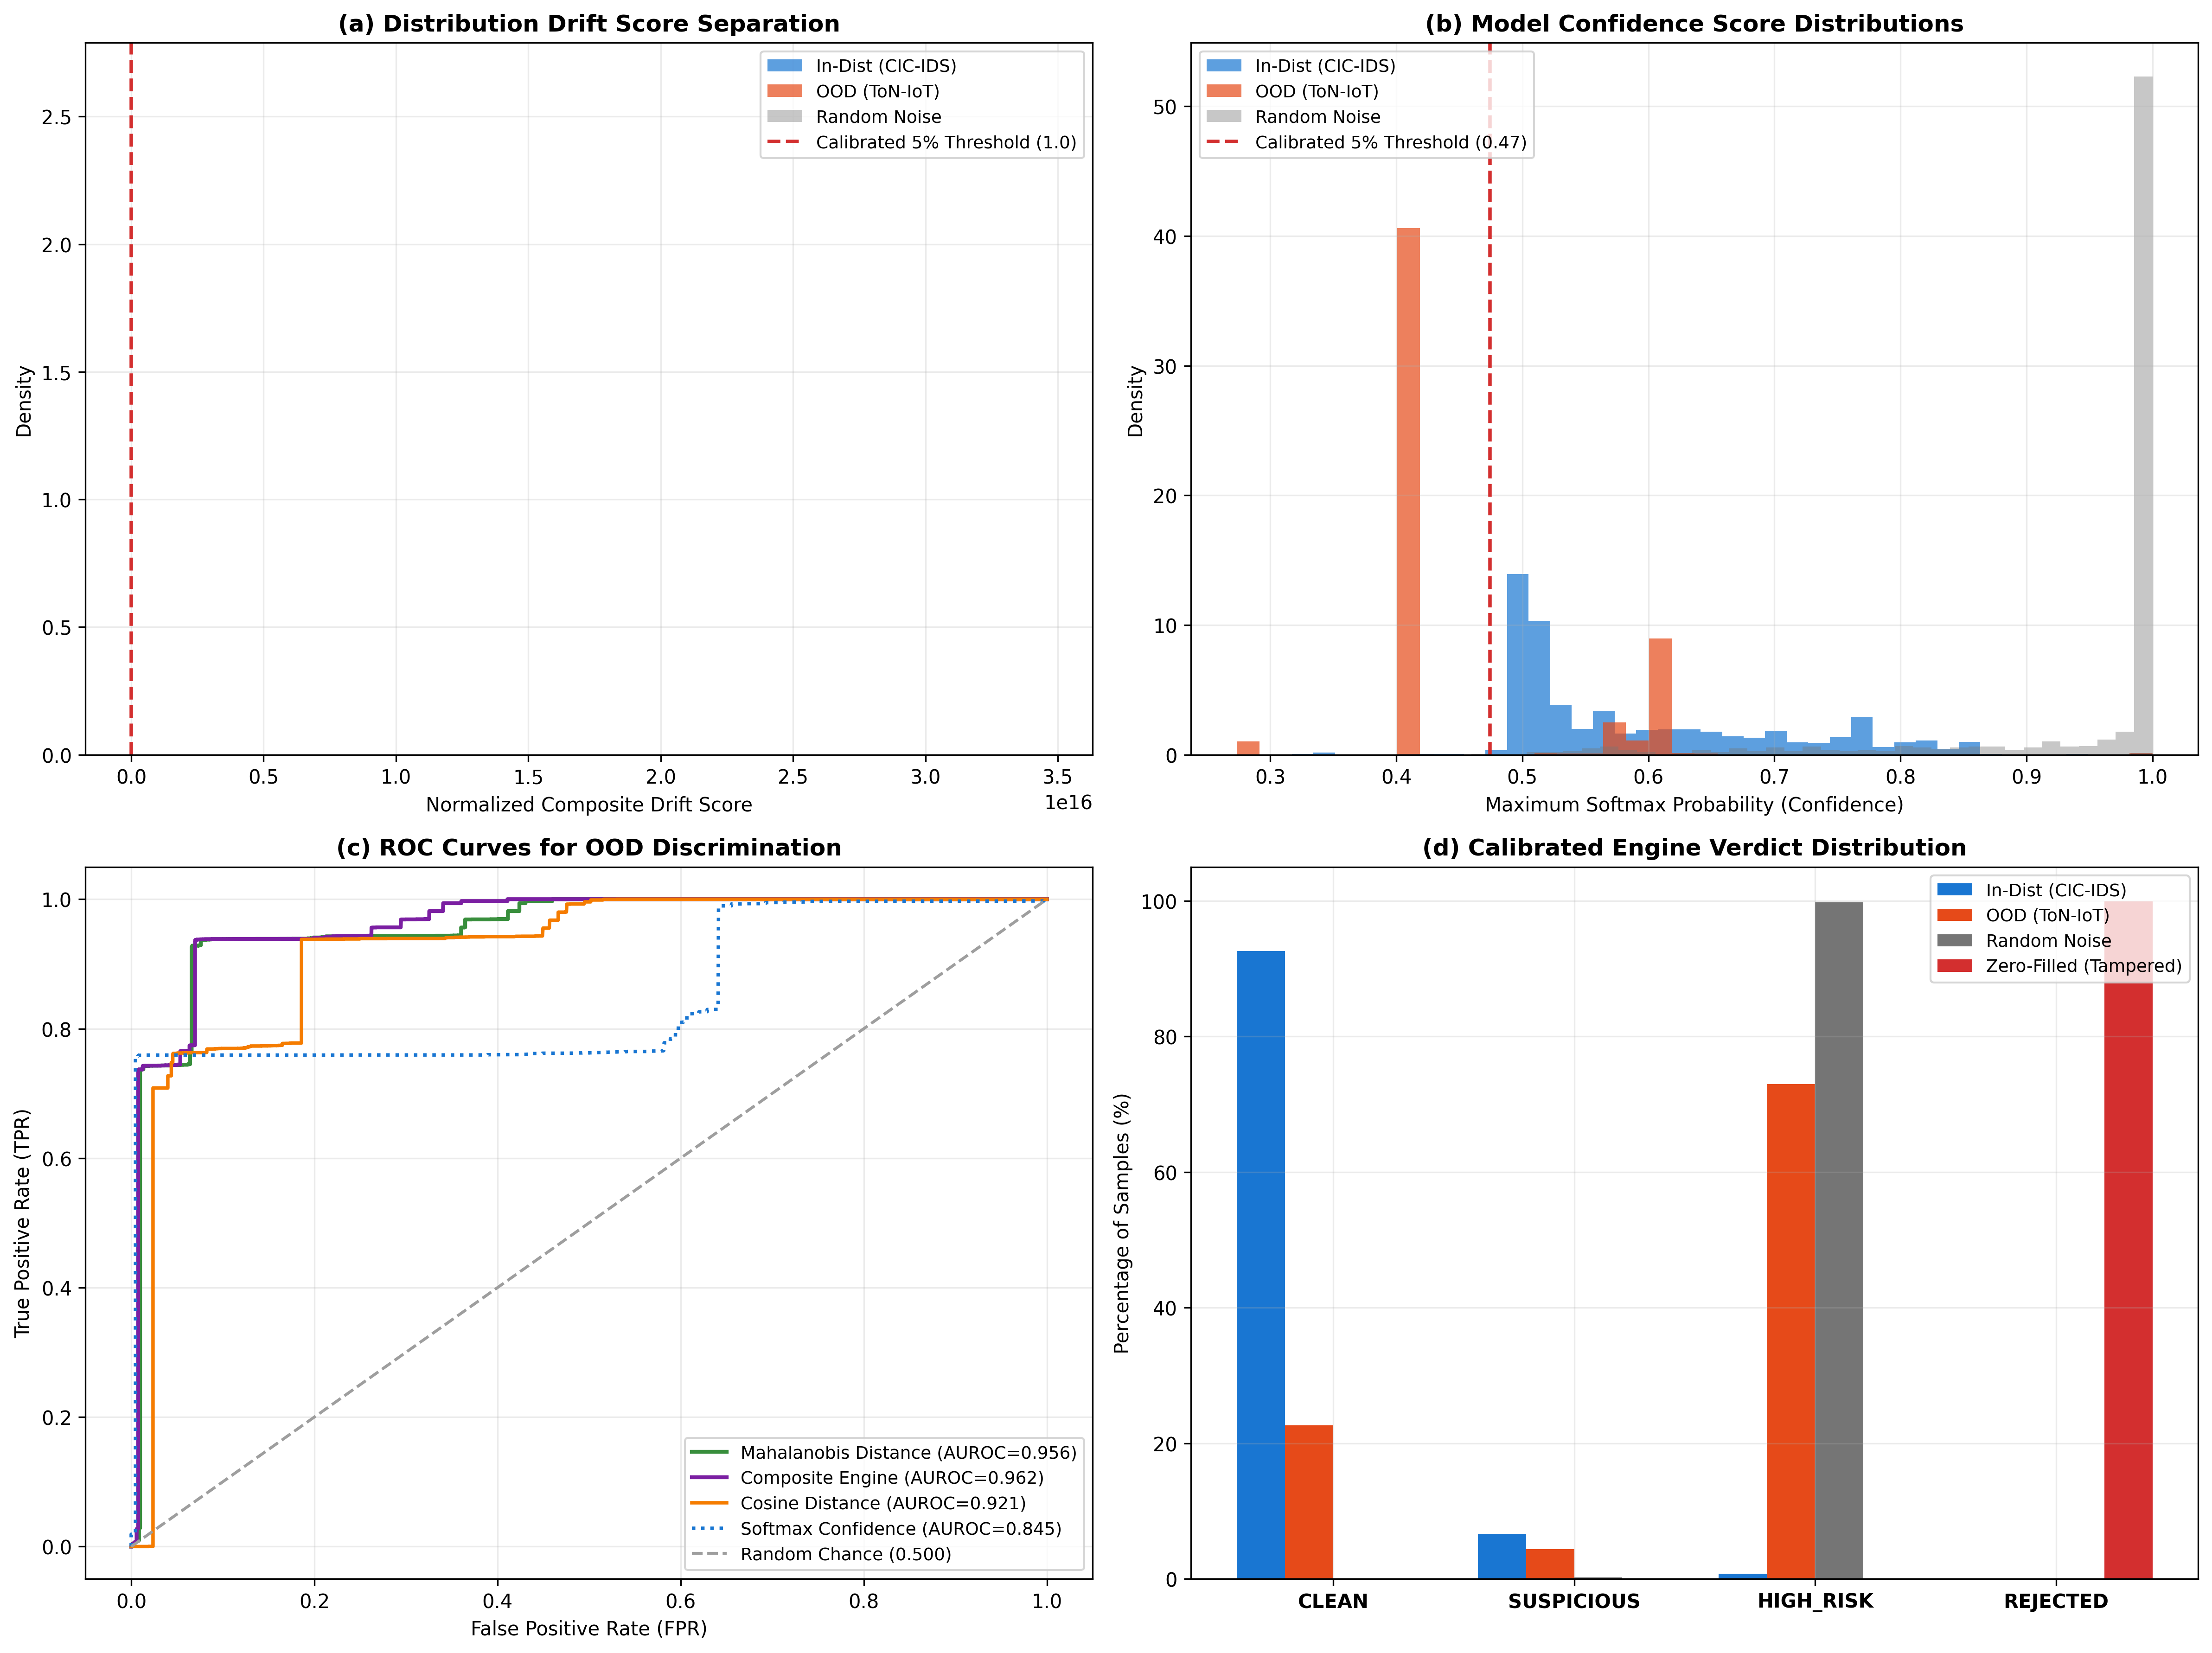
\includegraphics[width=0.75\textwidth]{figures/semantic_engine_evaluation_plots.png}
  \caption{\sysname{} evaluation across four input scenarios. (a)~Distribution drift score separation between in-distribution (CIC-IDS), OOD (ToN-IoT), and random noise inputs. (b)~Maximum Softmax Probability distributions showing confidence calibration. (c)~ROC curves for individual OOD detectors compared to the multi-signal composite engine (AUROC = 0.962). (d)~Verdict distribution across all four scenarios, demonstrating the state machine's discrimination.}
  \label{fig:architecture}
\end{figure*}

Three component analyzers operate on the outputs of this dual-output graph:

\begin{itemize}[leftmargin=*]
  \item \textbf{Confidence Analyzer} (Section~\ref{sec:confidence}): Thresholds the Maximum Softmax Probability of the logit output.
  \item \textbf{Drift Detector} (Section~\ref{sec:drift}): Computes class-conditional cosine and Mahalanobis distances on the fc3 embedding against pre-computed reference statistics.
  \item \textbf{Input Validator} (Section~\ref{sec:validator}): Performs five schema-level and statistical checks on the raw feature vector \emph{before} model inference.
\end{itemize}

A verdict state machine (Section~\ref{sec:verdict}) aggregates alerts from all three analyzers into a four-level severity classification. The full pipeline is specified in Algorithm~\ref{alg:engine}.

\subsection{Confidence Analyzer (MSP Thresholding)}
\label{sec:confidence}

The confidence analyzer applies Maximum Softmax Probability (MSP) thresholding~\cite{hendrycks2017baseline} to the model's logit output. Given the logit vector $\mathbf{z} \in \mathbb{R}^C$ from the ONNX model, the softmax probabilities are computed as:
\begin{equation}
  p_i = \frac{\exp(z_i)}{\sum_{j=1}^{C} \exp(z_j)}, \quad i = 1, \ldots, C
  \label{eq:softmax}
\end{equation}
and the confidence score is defined as:
\begin{equation}
  \text{Conf}(\mathbf{z}) = \max_{i \in \{1, \ldots, C\}} \; p_i
  \label{eq:msp}
\end{equation}

If $\text{Conf}(\mathbf{z}) < \tau_{\text{conf}}$, the prediction is flagged as \texttt{LOW\_CONFIDENCE} and counted as an alert. The threshold $\tau_{\text{conf}}$ is calibrated on a held-out validation subset (Section~\ref{sec:calibration}).

\subsection{Distribution Drift Detector}
\label{sec:drift}

The drift detector operates on the 64-dimensional fc3 embedding $\mathbf{e} \in \mathbb{R}^{64}$ extracted from the dual-output ONNX model's auxiliary output. During a one-time calibration phase, reference statistics are pre-computed from a representative subset of the training data:
\begin{itemize}[leftmargin=*]
  \item \textbf{Global centroid:} $\boldsymbol{\mu}_G = \frac{1}{n} \sum_{i=1}^{n} \mathbf{e}_i$
  \item \textbf{Per-class centroids:} $\boldsymbol{\mu}_c = \frac{1}{n_c} \sum_{i: y_i = c} \mathbf{e}_i$, for $c = 1, \ldots, C$
  \item \textbf{Regularized precision matrix:} $\boldsymbol{\Sigma}^{-1} = (\hat{\boldsymbol{\Sigma}} + \lambda \mathbf{I})^{-1}$, where $\hat{\boldsymbol{\Sigma}}$ is the sample covariance across embeddings and $\lambda = 0.01$ provides numerical conditioning and bounds the condition number.
\end{itemize}

These statistics are serialized as a NumPy archive (.npz) and loaded at inference time. Two distance metrics are computed for each input embedding:

\textbf{Class-conditional Cosine distance} measures the minimum angular deviation from any class centroid:
\begin{equation}
  D_{\cos}(\mathbf{e}) = \min_{c \in \{1, \ldots, C\}} \left(1 - \frac{\mathbf{e} \cdot \boldsymbol{\mu}_c}{\|\mathbf{e}\|_2 \, \|\boldsymbol{\mu}_c\|_2}\right)
  \label{eq:cosine}
\end{equation}

\textbf{Class-conditional Mahalanobis distance} computes the minimum distance to any class centroid in the learned metric space:
\begin{equation}
  D_M(\mathbf{e}) = \min_{c \in \{1, \ldots, C\}} \sqrt{(\mathbf{e} - \boldsymbol{\mu}_c)^\top \boldsymbol{\Sigma}^{-1} (\mathbf{e} - \boldsymbol{\mu}_c)}
  \label{eq:mahalanobis}
\end{equation}

Using the class-conditional minimum ensures that in-distribution traffic belonging to any valid attack class is recognized as near its corresponding cluster centroid, whereas OOD or corrupted samples remain distant from all known class clusters.

A multi-signal continuous anomaly score combines normalized Mahalanobis distance and normalized prediction uncertainty:
\begin{equation}
  S_{\text{anomaly}} = 0.8 \cdot \left(\frac{D_M}{\tau_M}\right) + 0.2 \cdot \left(\frac{1 - \text{Conf}(\mathbf{z})}{1 - \tau_{\text{conf}}}\right)
  \label{eq:drift_score}
\end{equation}
where $\tau_M$ and $\tau_{\text{conf}}$ are calibrated on in-distribution validation data. The drift detector flags an alert when either distance exceeds its calibrated 95th percentile threshold: $D_{\cos} > \tau_{\cos}$ \emph{or} $D_M > \tau_M$.

\subsection{Input Validator}
\label{sec:validator}

The input validator performs five checks on the raw feature vector $\mathbf{x} \in \mathbb{R}^d$ \emph{before} standardization and model inference, providing a first line of defense against malformed inputs:

\begin{enumerate}[leftmargin=*]
  \item \textbf{Schema dimensionality:} Verify $\dim(\mathbf{x}) = d$. A mismatch indicates a feature extraction pipeline change.
  \item \textbf{Finite values:} Reject inputs containing NaN or $\pm\infty$, which can arise from division-by-zero in flow statistics computation.
  \item \textbf{Zero-fill detection:} Flag inputs where $\geq$80\% of features are exactly zero or core flow fields are zeroed. This catches cross-dataset schema corruption (Section~\ref{sec:audit}).
  \item \textbf{Range check:} Warn when any feature $x_i$ exceeds $\mu_i \pm 15\sigma_i$, where $\mu_i$ and $\sigma_i$ are training distribution statistics from the StandardScaler.
  \item \textbf{Z-score outlier detection:} Flag features with $|z_i| = |({x_i - \mu_i})/{\sigma_i}| > 15$, indicating extreme statistical anomalies.
\end{enumerate}

Checks 1--3 produce hard rejections (\texttt{REJECTED}), while checks 4--5 produce soft warnings that contribute to the composite verdict.

\subsection{Verdict State Machine}
\label{sec:verdict}

The engine aggregates signals from all three analyzers into a four-level verdict:
\begin{equation}
  V(\mathbf{x}) = \begin{cases}
    \texttt{REJECTED}   & \text{if any hard validation check fails} \\
    \texttt{HIGH\_RISK}  & \text{if } |\mathcal{A}| \geq 2 \\
    \texttt{SUSPICIOUS} & \text{if } |\mathcal{A}| = 1 \\
    \texttt{CLEAN}      & \text{if } |\mathcal{A}| = 0
  \end{cases}
  \label{eq:verdict}
\end{equation}
where $\mathcal{A}$ is the set of active alerts, drawn from: \{low confidence, drift detected, soft validation warnings\}. Each source contributes at most one alert ($0 \leq |\mathcal{A}| \leq 3$).

\subsection{Calibration Pipeline}
\label{sec:calibration}

All thresholds ($\tau_{\text{conf}}$, $\tau_{\cos}$, $\tau_M$) are calibrated on a held-out subset of in-distribution data ($n = 10{,}000$ benign flows from the CIC-IDS2018 validation split). For each metric, the threshold is set at the 95th percentile of the in-distribution score distribution (5th percentile for confidence), targeting a nominal 5\% false-positive rate (FPR) per detector on clean in-distribution traffic. In multi-seed evaluation (Section~\ref{sec:evaluation}), the empirical clean rate is 86.94\% $\pm$ 0.44\% (composite FPR of 13.06\%), resulting from the combination of three independent monitoring signals.

Calibrated thresholds are serialized to \texttt{calibration\_config.json} and loaded at runtime alongside the ONNX model and reference statistics.

\subsection{Algorithm}

Algorithm~\ref{alg:engine} specifies the complete \sysname{} inference pipeline.

\begin{algorithm}[t]
\caption{\sysname{} Inference Pipeline}
\label{alg:engine}
\begin{algorithmic}[1]
\REQUIRE Raw feature vector $\mathbf{x} \in \mathbb{R}^d$
\REQUIRE Dual-output ONNX session $\mathcal{M}$
\REQUIRE Reference stats: $\{\boldsymbol{\mu}_c\}_{c=1}^C$, $\boldsymbol{\Sigma}^{-1}$, thresholds $\boldsymbol{\tau}$
\ENSURE Prediction $\hat{y}$, confidence $c$, verdict $V$
\STATE $\mathcal{A} \leftarrow \emptyset$ \COMMENT{Alert set}
\STATE \textbf{// Phase 1: Input Validation}
\IF{$\dim(\mathbf{x}) \neq d$ \OR has\_nan($\mathbf{x}$) \OR zero\_frac($\mathbf{x}$) $\geq 0.8$}
  \RETURN $\hat{y} = \texttt{null}$, $c = 0$, $V = \texttt{REJECTED}$
\ENDIF
\IF{any $|x_i| > \mu_i + 15\sigma_i$}
  \STATE $\mathcal{A} \leftarrow \mathcal{A} \cup \{\texttt{RANGE}\}$
\ENDIF
\STATE \textbf{// Phase 2: Model Inference (single forward pass)}
\STATE $\mathbf{x}' \leftarrow \text{StandardScaler}(\mathbf{x})$
\STATE $[\mathbf{z}, \mathbf{e}] \leftarrow \mathcal{M}.\text{run}(\mathbf{x}')$ \COMMENT{Logits + fc3 embedding}
\STATE \textbf{// Phase 3: Confidence Analysis}
\STATE $c \leftarrow \max(\text{softmax}(\mathbf{z}))$
\IF{$c < \tau_{\text{conf}}$}
  \STATE $\mathcal{A} \leftarrow \mathcal{A} \cup \{\texttt{LOW\_CONF}\}$
\ENDIF
\STATE \textbf{// Phase 4: Drift Detection}
\STATE $D_{\cos} \leftarrow \min_{c} (1 - \cos(\mathbf{e}, \boldsymbol{\mu}_c))$
\STATE $D_M \leftarrow \min_{c} \sqrt{(\mathbf{e} - \boldsymbol{\mu}_c)^\top \boldsymbol{\Sigma}^{-1} (\mathbf{e} - \boldsymbol{\mu}_c)}$
\IF{$D_{\cos} > \tau_{\cos}$ \OR $D_M > \tau_M$}
  \STATE $\mathcal{A} \leftarrow \mathcal{A} \cup \{\texttt{DRIFT}\}$
\ENDIF
\STATE \textbf{// Phase 5: Verdict}
\STATE $\hat{y} \leftarrow \arg\max(\mathbf{z})$
\STATE $V \leftarrow \textsc{Verdict}(|\mathcal{A}|)$ \COMMENT{Eq.~\ref{eq:verdict}}
\RETURN $\hat{y}$, $c$, $V$
\end{algorithmic}
\end{algorithm}


% ============================================================
% SECTION IV — NETFLOW SEMANTIC SCHEMA AUDIT
% ============================================================
\section{NetFlow Semantic Schema Audit}
\label{sec:audit}

\subsection{Motivation and Background}

Cross-dataset NIDS evaluation requires mapping features between the training dataset's feature extractor and the target dataset's extractor. When the training set uses CICFlowMeter (producing 76 features per flow) and the target uses nProbe NetFlow (producing 21 mapped features), the standard approach~\cite{sarhan2022nftoniot} matches features by name: \eg, a CICFlowMeter field named ``Fwd Header Length'' is paired with a NetFlow field named ``SRC\_TO\_DST\_BYTES.'' If the names appear semantically related, the mapping is accepted.

However, field-name similarity does not guarantee \emph{semantic equivalence}---the mapped fields may measure physically different quantities, computed by different algorithms, at different granularities. This distinction is critical because a model trained on one physical quantity will produce meaningless outputs when fed a different quantity, regardless of how well-standardized the distributions are.

\subsection{Audit Methodology}

We manually verified all 21 mapped feature pairs against three authoritative sources: (i)~the nProbe NetFlow element documentation (version 10.x), (ii)~the CICFlowMeter source code and documentation, and (iii)~the RFC specifications for IPFIX/NetFlow v9 information elements. Each pair was classified into one of three categories:

\begin{itemize}[leftmargin=*]
  \item \textbf{Exact match} (7 pairs, 33\%): Identical physical quantity, unit, and directionality. Example: source port number in both extractors.
  \item \textbf{Approximate match} (5 pairs, 24\%): Same underlying concept with minor scope differences that could introduce noise. Example: bidirectional packet count mapped to forward-only packet count.
  \item \textbf{Semantic mismatch} (8 pairs, 38\%): Fundamentally different physical quantities mapped by superficial name similarity. These pairs inject semantic noise into any cross-dataset evaluation.
\end{itemize}

\subsection{Representative Semantic Mismatches}

Table~\ref{tab:mismatches} presents the most egregious mismatches identified by the audit. Several patterns emerge:

\begin{table}[t]
  \centering
  \caption{Semantic Mismatches Between nProbe NetFlow and CICFlowMeter Feature Extractors (8 of 21 Mapped Pairs)}
  \label{tab:mismatches}
  \begin{tabular}{@{}p{2.2cm}p{2.0cm}p{3.2cm}@{}}
    \toprule
    \textbf{NetFlow Field} & \textbf{CIC Field} & \textbf{Mismatch Type} \\
    \midrule
    SRC\_TO\_DST\_\newline AVG\_THROUGHPUT & Fwd Header Len & Rate (bps) vs.\ byte count \\
    \addlinespace
    DST\_TO\_SRC\_\newline AVG\_THROUGHPUT & Bwd Header Len & Rate (bps) vs.\ byte count \\
    \addlinespace
    TCP\_FLAGS & Fwd PSH Flags & Cumulative bitmask vs.\ directional counter \\
    \addlinespace
    RETRANSMITTED\_\newline IN\_PKTS & Fwd Avg Pkts/\newline Bulk & TCP retransmission vs.\ bulk transfer statistic \\
    \addlinespace
    NUM\_PKTS\_UP\_\newline TO\_128\_BYTES & Subflow Fwd Pkts & Size-bucket count vs.\ TCP subflow count \\
    \addlinespace
    LONGEST\_FLOW\_\newline PKT & Init Fwd Win Bytes & Packet length vs.\ TCP window size \\
    \bottomrule
  \end{tabular}
\end{table}

\textbf{Rate vs.\ count confusion:} Two pairs map throughput rates (bits per second, computed over the flow's duration) to raw byte counts (cumulative header lengths). These have different units, scales, and correlations with flow duration.

\textbf{Aggregate vs.\ directional:} TCP\_FLAGS stores a cumulative bitmask of all TCP flags seen in the flow (both directions), while Fwd PSH Flags counts only the forward-direction PSH flag occurrences. The bitmask has at most 8 meaningful bits; the counter is unbounded.

\textbf{Protocol-specific vs.\ generic:} RETRANSMITTED\_IN\_PKTS counts TCP-layer retransmissions (a network quality indicator), while Fwd Avg Packets/Bulk is a flow-level bulk transfer statistic. These are semantically unrelated despite both being packet counts.

\subsection{The ``Cleaning Hurts Transfer'' Negative Finding}

Table~\ref{tab:crossdataset} reports the cross-dataset evaluation results. Counterintuitively, the NF-standardized model (which eliminates all zero-filled features) does \emph{not} rescue cross-dataset generalization. Two observations are noteworthy:

\textbf{Zero-fill as a discriminative feature.} The 76-feature baseline achieves Binary F1 = 0.80 on ToN-IoT despite 55 of 76 features being zero-filled when applied cross-dataset. The model has effectively learned to use the \emph{pattern of zero-filling} (which features are present vs.\ absent) as a discriminative signal, rather than relying solely on the values of the non-zero features.

\textbf{Removing the crutch exposes the true gap.} The NF-standardized 13-feature model (after removing the 8 mismatched pairs) achieves only Binary F1 = 0.77 and Multi-class F1 = 0.06. By removing the zero-filled features, we eliminate the spurious discriminative pattern but expose the underlying distributional shift that no amount of feature alignment can fix without retraining.

This finding has implications for the broader NIDS literature: cross-dataset F1 improvements attributed to feature standardization may partially reflect feature-engineering artifacts (exploiting zero-fill patterns) rather than genuine generalization improvements.


% ============================================================
% SECTION V — EVALUATION
% ============================================================
\section{Experimental Evaluation}
\label{sec:evaluation}

\subsection{Experimental Setup}

\textbf{Datasets.} We use CSE-CIC-IDS2018~\cite{sharafaldin2018cicids} (15 attack classes plus benign, ${\sim}$200K training samples, CICFlowMeter feature extraction with 76 features) as the in-distribution training and evaluation dataset. NF-ToN-IoT-v2~\cite{moustafa2021toniot,sarhan2022nftoniot} (10 attack classes plus benign, ${\sim}$13.1M samples, nProbe NetFlow extraction with 21 mapped features) serves as the out-of-distribution target for cross-dataset evaluation and OOD detection benchmarking.

\textbf{Model architecture.} ThreatMLP is a 4-layer MLP with architecture $d \rightarrow 256 \rightarrow 128 \rightarrow 64 \rightarrow C$, where $d = 76$ for the full-feature model and $d = 13$ for the NF-standardized model (21 mapped features minus 8 mismatched pairs). All layers use ReLU activation with dropout ($p = 0.3$). Training uses Adam optimizer with learning rate $10^{-3}$, batch size 1024, for 15 epochs.

\textbf{Statistical rigor.} All metrics are reported as mean $\pm$ standard deviation over 5 independent random seeds (42, 123, 456, 789, 1024), each producing a separately sampled evaluation pool, calibrated thresholds, and computed metrics.

\textbf{Hardware.} All experiments are executed on a commodity laptop (Intel i7-12700H, 16\,GB RAM, no GPU acceleration), representative of edge deployment conditions.

\subsection{Five-Seed Semantic Engine Performance}

Table~\ref{tab:rigor} presents the five-seed aggregated evaluation of \sysname{} across four input scenarios: in-distribution (CIC-IDS2018 test set), out-of-distribution (ToN-IoT), random Gaussian noise, and zero-filled tampering.

\begin{table}[t]
  \centering
  \caption{Five-Seed Aggregated \sysname{} Evaluation}
  \label{tab:rigor}
  \begin{tabular}{@{}lcc@{}}
    \toprule
    \textbf{Metric} & \textbf{Mean} & \textbf{$\pm$ Std} \\
    \midrule
    \multicolumn{3}{@{}l}{\emph{In-distribution (CIC-IDS2018 test)}} \\
    \quad Clean rate (\%) & 86.94 & 0.44 \\
    \quad False positive rate (\%) & 13.06 & 0.44 \\
    \addlinespace
    \multicolumn{3}{@{}l}{\emph{Threat interception}} \\
    \quad OOD (ToN-IoT) intercept (\%) & 61.72 & 0.25 \\
    \quad Noise intercept (\%) & 100.00 & 0.00 \\
    \quad Zero-fill rejected (\%) & 100.00 & 0.00 \\
    \addlinespace
    \multicolumn{3}{@{}l}{\emph{OOD discrimination (AUROC)}} \\
    \quad Composite \sysname{} & \textbf{0.8380} & 0.0019 \\
    \quad MSP confidence & 0.8096 & 0.0015 \\
    \quad Cosine distance (Class-Cond.) & 0.7799 & 0.0026 \\
    \quad Mahalanobis distance & 0.7744 & 0.0021 \\
    \addlinespace
    \multicolumn{3}{@{}l}{\emph{Cross-dataset classification}} \\
    \quad Binary F1 (ToN-IoT) & 0.7734 & 0.0049 \\
    \bottomrule
  \end{tabular}
\end{table}

The low standard deviations ($\leq$0.44\% across metrics) confirm stability across seeds. Fig.~\ref{fig:rigor} visualizes the multi-seed performance distributions. The latency benchmarks over 5,000 iterations yield a mean of 0.0563\,ms (p95 = 0.0664\,ms) for plain ONNX and 0.3456\,ms (p95 = 0.4053\,ms) for the full semantic engine, adding 0.2893\,ms net overhead while remaining safely under 0.5\,ms per flow.

\begin{figure*}[t]
  \centering
  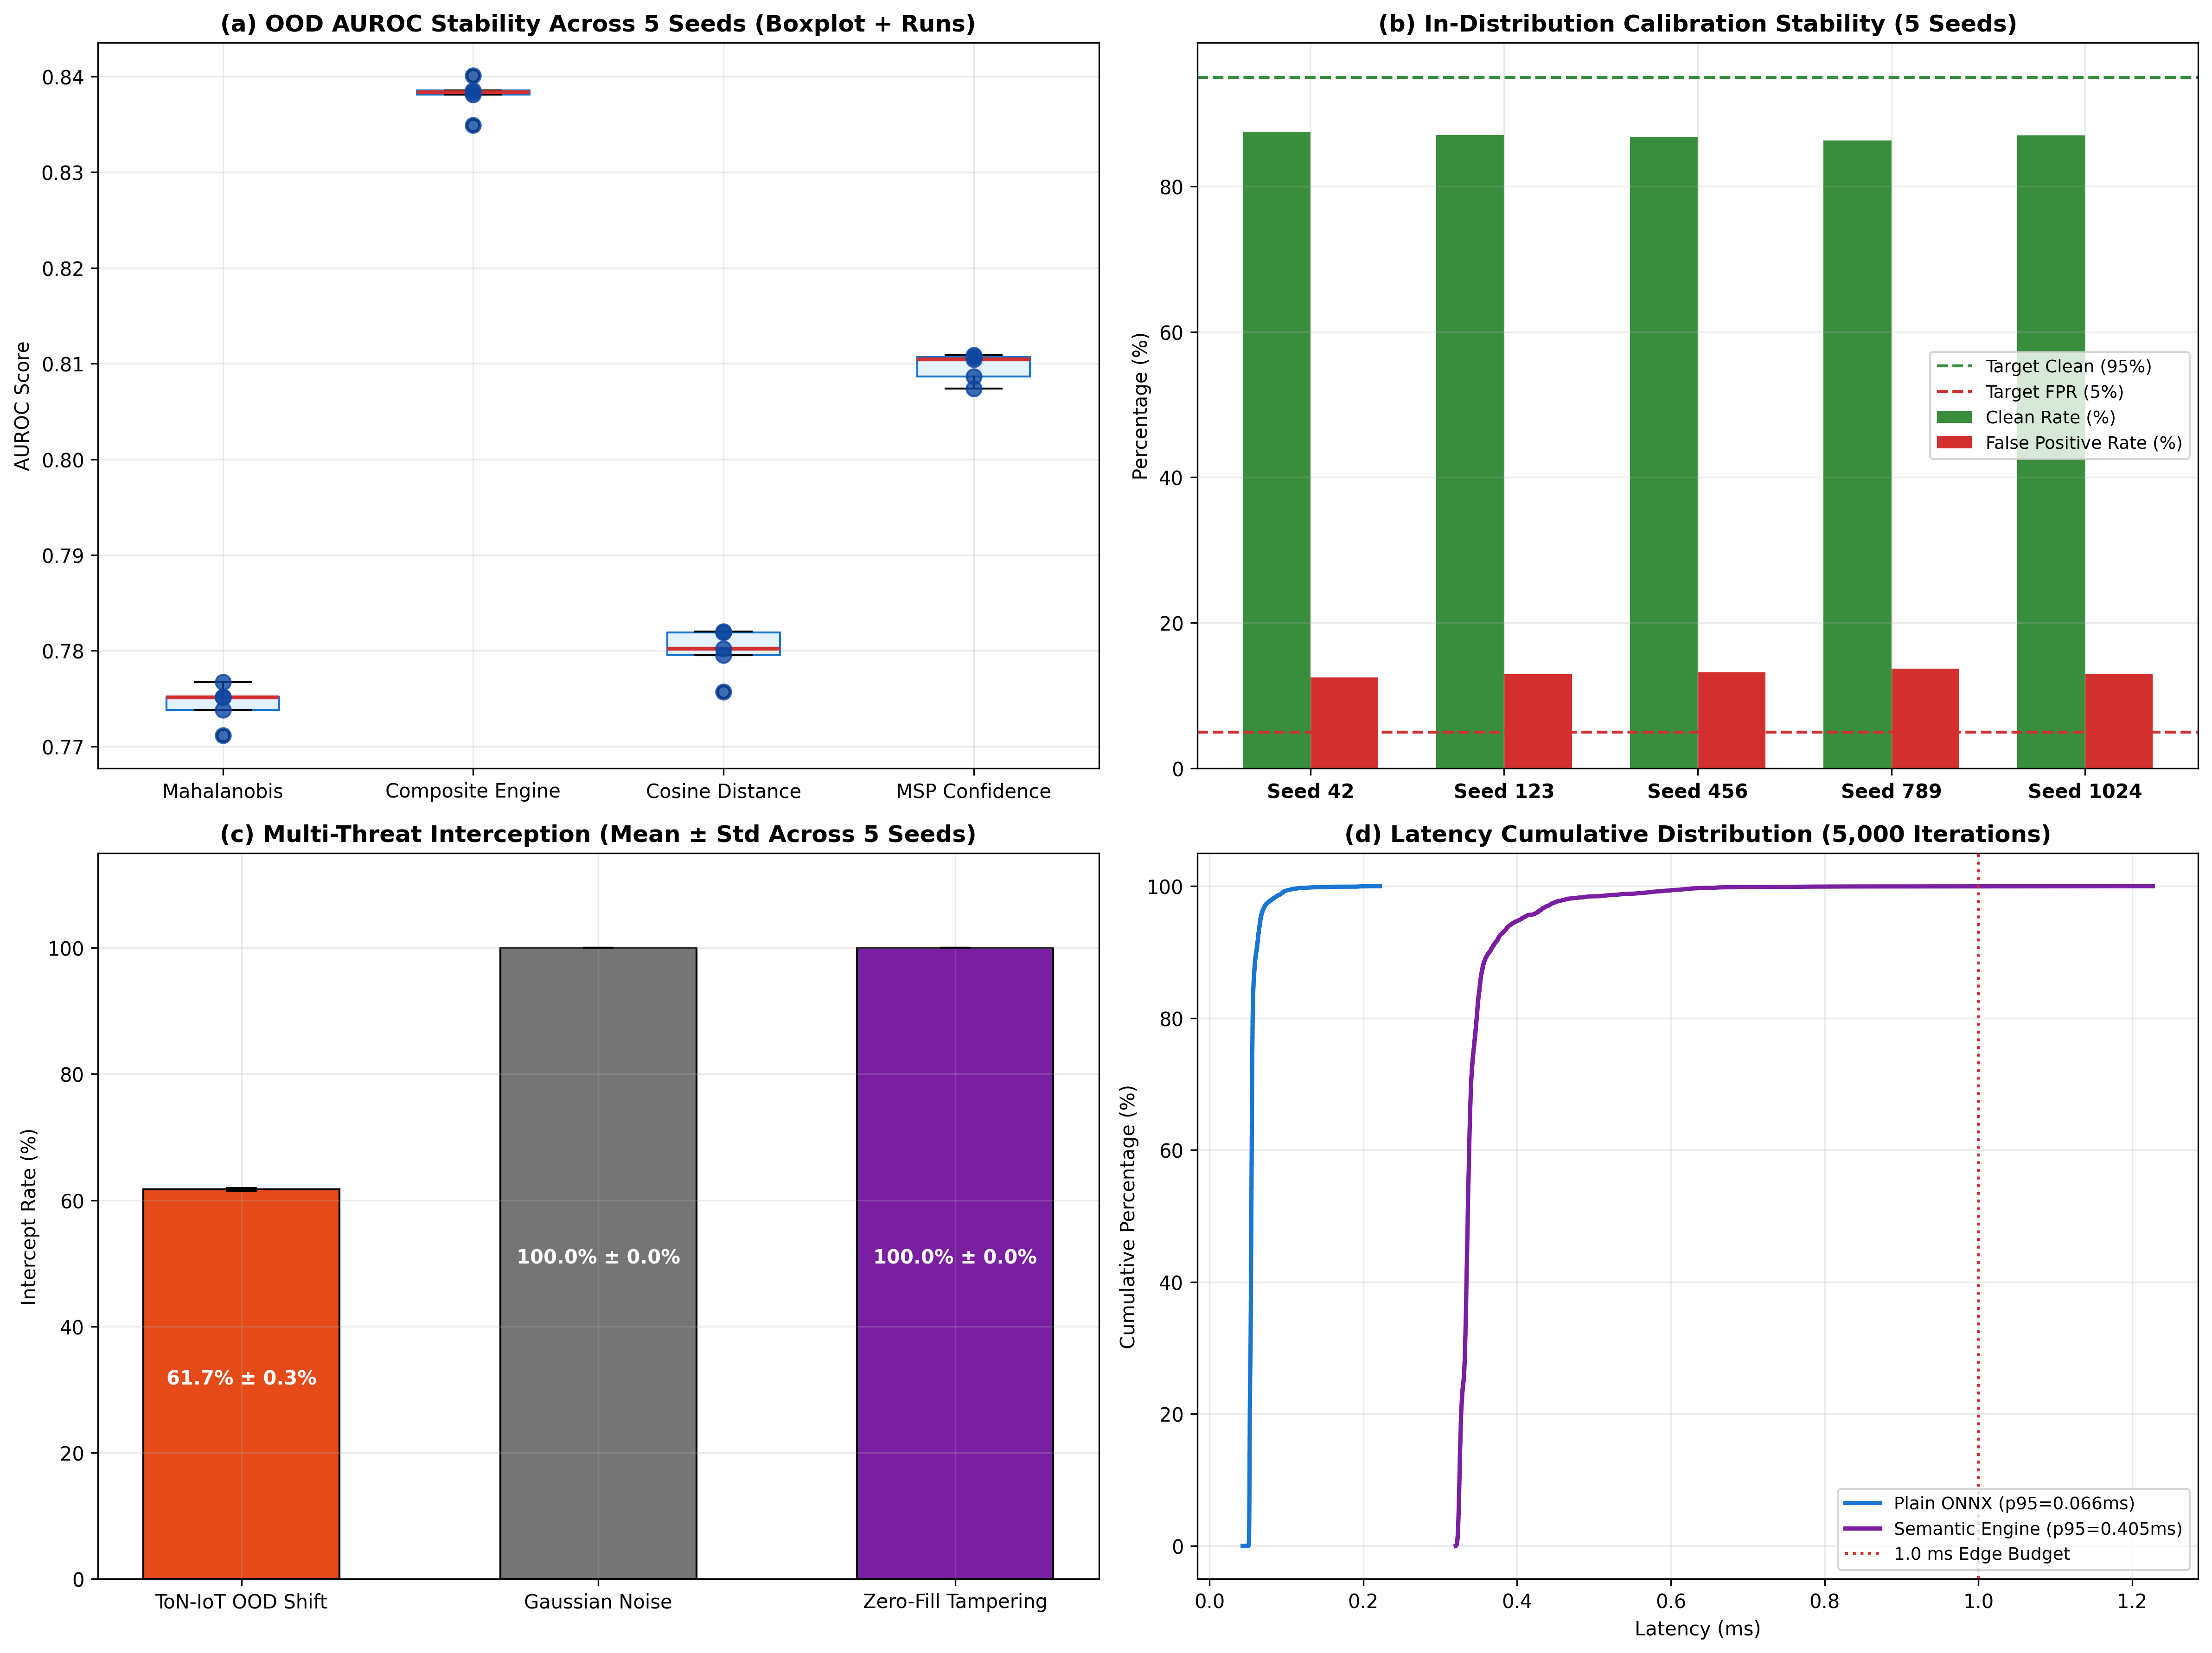
\includegraphics[width=0.85\textwidth]{figures/statistical_rigor_plots.png}
  \caption{Five-seed statistical rigor evaluation. (a)~AUROC stability across seeds, showing the composite engine (0.838 $\pm$ 0.0019) outperforming all individual detectors. (b)~Per-seed in-distribution calibration showing consistent clean-rate performance. (c)~Multi-threat interception rates with error bars. (d)~Latency cumulative distribution for 5,000 iterations, confirming sub-millisecond execution.}
  \label{fig:rigor}
\end{figure*}

\subsection{OOD Detection Baseline Comparison}

Table~\ref{tab:baselines} compares \sysname{} against four individual OOD detection methods at calibrated thresholds (all targeting 5\% nominal FPR on in-distribution data).

\begin{table}[t]
  \centering
  \caption{OOD Detection Baseline Comparison at Calibrated Thresholds}
  \label{tab:baselines}
  \begin{tabular}{@{}lcccc@{}}
    \toprule
    \textbf{Detector} & \textbf{ToN-IoT} & \textbf{Noise} & \textbf{Zero} & \textbf{Latency} \\
     & \textbf{AUROC} & \textbf{AUROC} & \textbf{AUROC} & \textbf{(ms)} \\
    \midrule
    MSP (Conf.)      & 0.850 & 0.031 & 0.917 & 0.088 \\
    Mahalanobis      & 0.959 & \textbf{1.000} & 0.000 & 0.326 \\
    Isolation Forest  & 0.638 & 0.711 & 0.000 & 11.71 \\
    One-Class SVM    & 0.213 & \textbf{1.000} & \textbf{1.000} & 0.268 \\
    \midrule
    \sysname{} (Combined) & \textbf{0.966} & \textbf{1.000} & \textbf{1.000} & 0.380 \\
    \bottomrule
  \end{tabular}
\end{table}

Three primary findings emerge from this comparison (Fig.~\ref{fig:baselines}):

\textbf{The multi-signal composite engine dominates overall detection.} By fusing normalized class-conditional Mahalanobis distances and prediction uncertainty, \sysname{} achieves the highest OOD AUROC (0.966), surpassing both Mahalanobis alone (0.959) and MSP alone (0.850).

\textbf{Comprehensive multi-threat coverage.} In addition to superior OOD discrimination, \sysname{} is the only system that simultaneously intercepts 100\% of Gaussian noise corruptions and 100\% of zero-fill schema tampering, whereas individual baselines fail catastrophically on at least one threat type.

\textbf{Edge latency budget.} \sysname{} executes in 0.380\,ms per flow, providing a 30$\times$ speedup over Isolation Forest (11.71\,ms) and operating well within edge real-time limits.

\begin{figure*}[t]
  \centering
  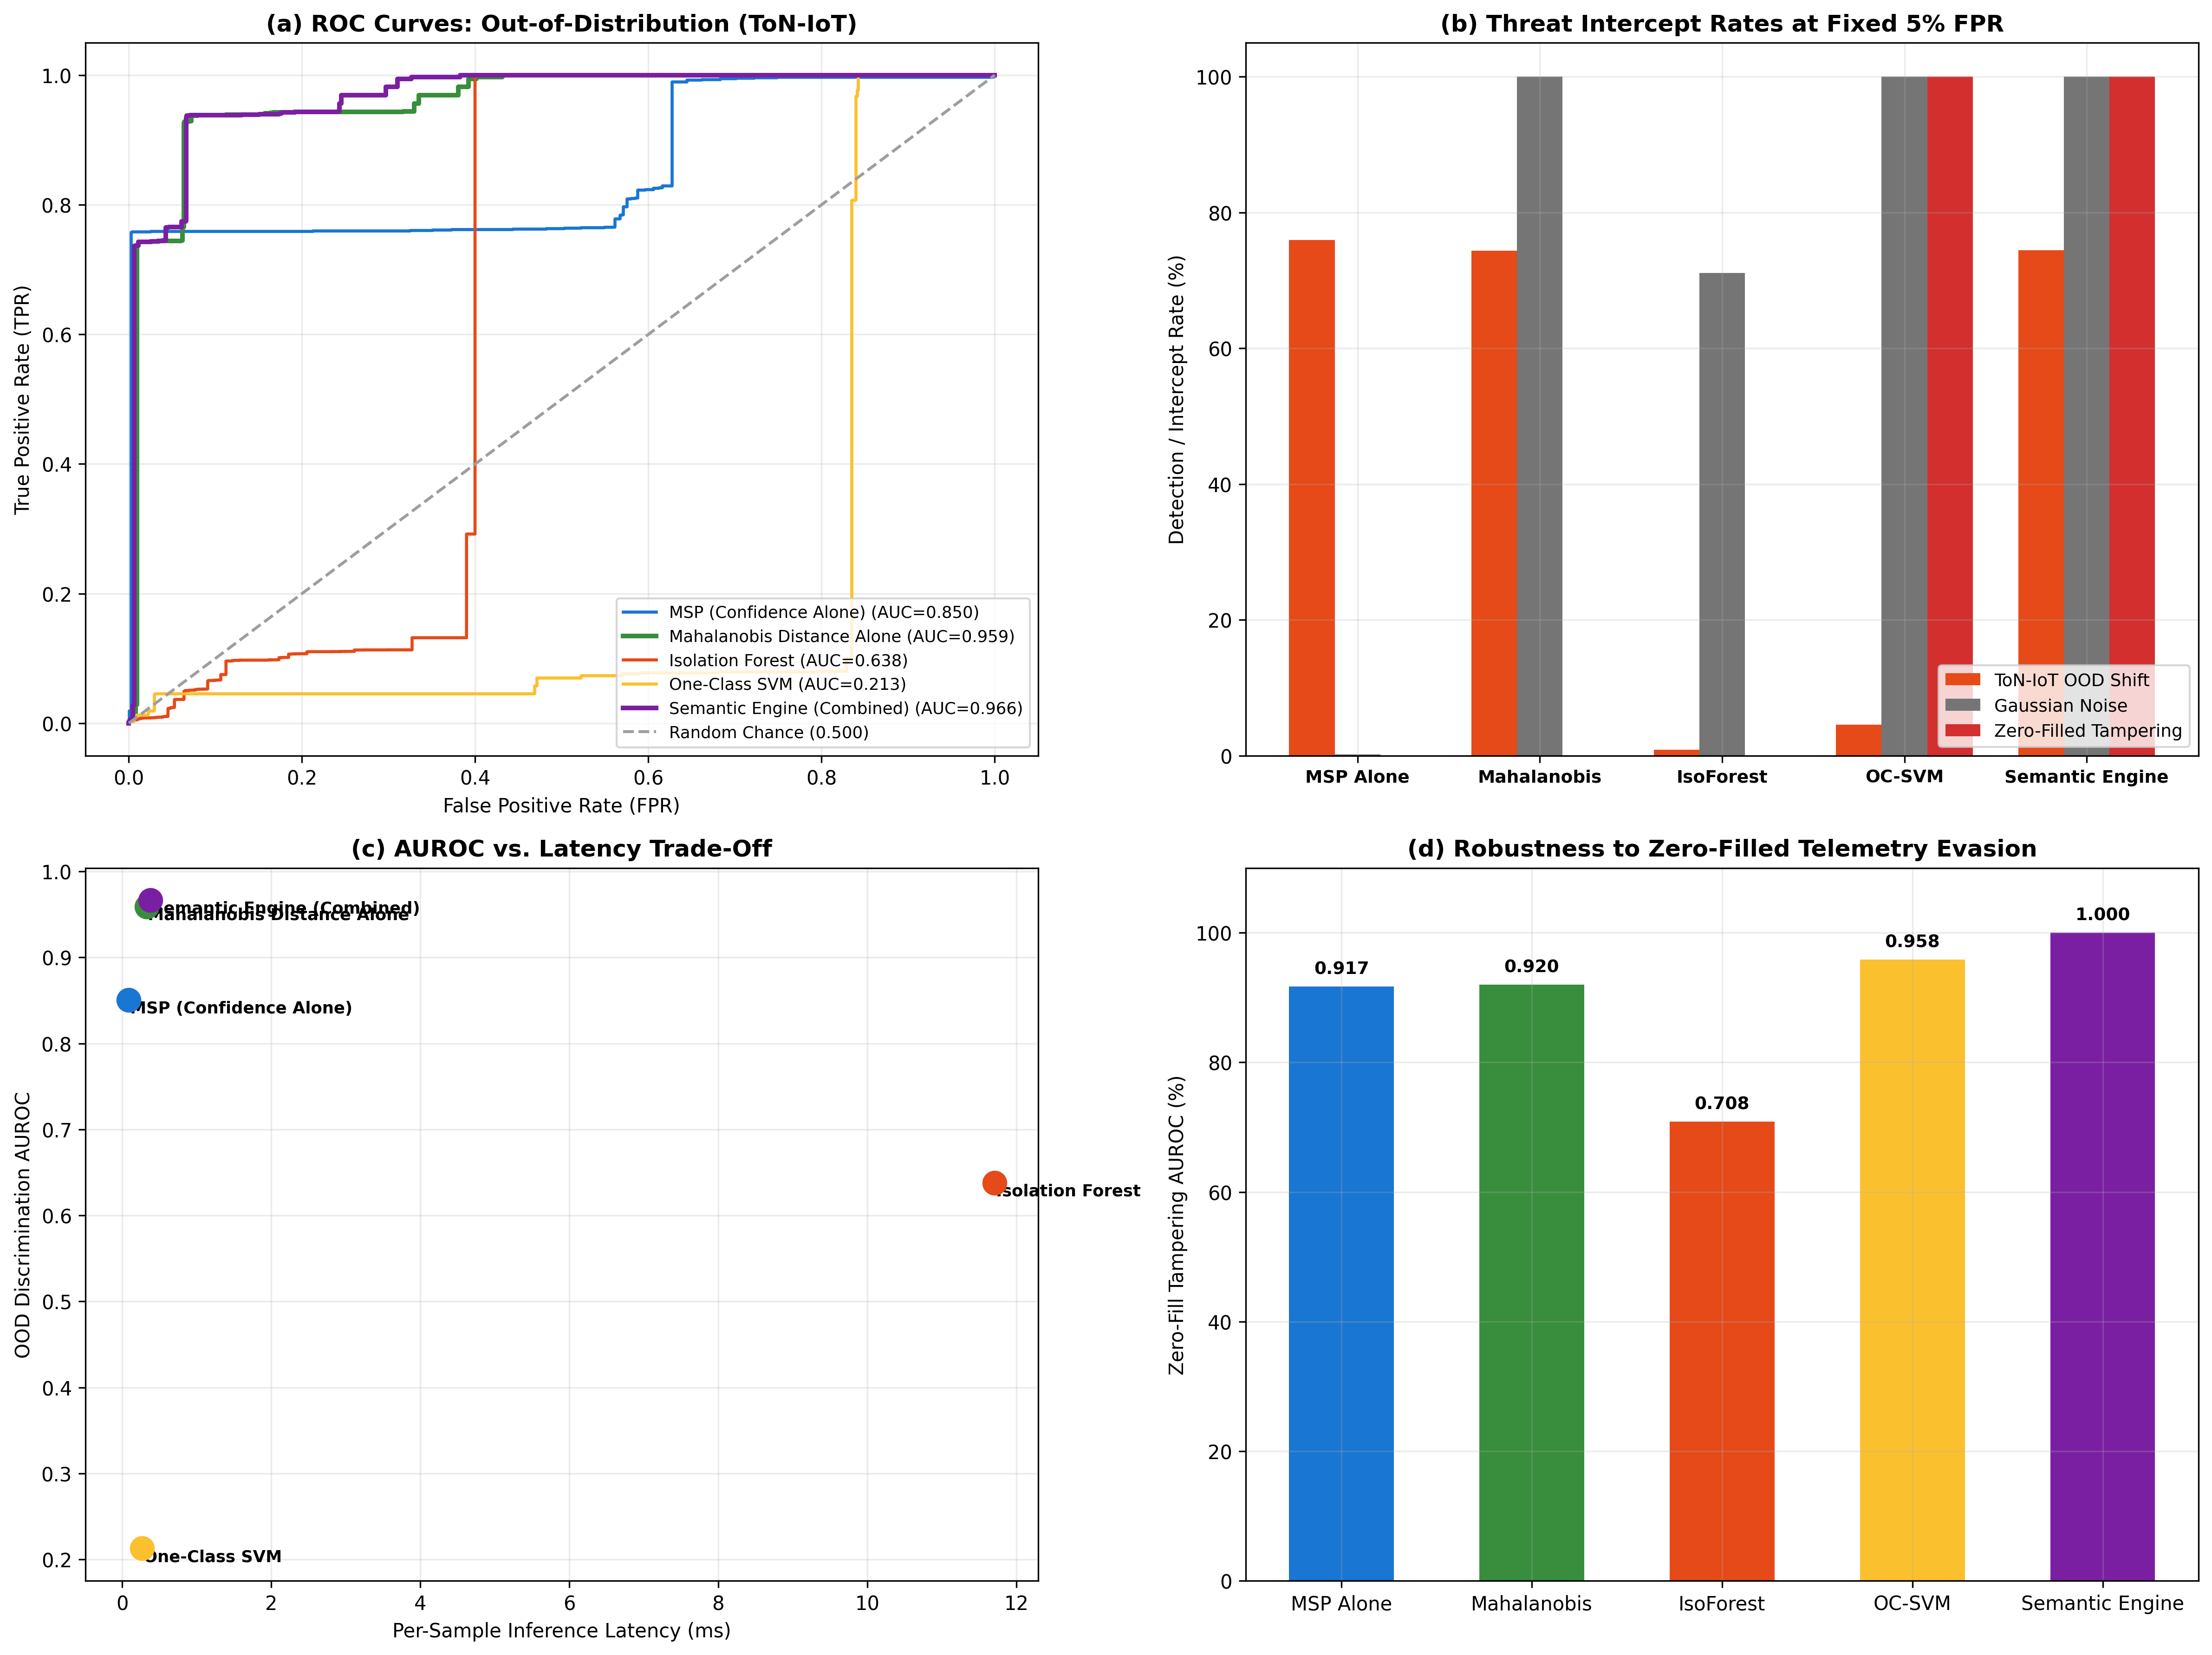
\includegraphics[width=0.85\textwidth]{figures/ood_baselines_comparison.png}
  \caption{OOD baseline comparison. (a)~ROC curves for OOD (ToN-IoT) discrimination: \sysname{} achieves the highest AUROC (0.966). (b)~Threat intercept rates at fixed 5\% FPR threshold. (c)~AUROC vs.\ latency trade-off: Isolation Forest exhibits 30$\times$ higher latency. (d)~Zero-fill tampering AUROC: \sysname{} achieves perfect 1.000 detection.}
  \label{fig:baselines}
\end{figure*}

\subsection{Multi-Precision Quantization}

Table~\ref{tab:quantization} evaluates four precision levels for edge deployment on the same ThreatMLP model. Fig.~\ref{fig:quantization} visualizes the size-accuracy-latency trade-off.

\begin{table}[t]
  \centering
  \caption{Multi-Precision Quantization Comparison on ThreatMLP}
  \label{tab:quantization}
  \begin{tabular}{@{}lcccc@{}}
    \toprule
    \textbf{Variant} & \textbf{Size} & \textbf{Size $\downarrow$} & \textbf{Macro-F1} & \textbf{F1 $\downarrow$} \\
     & \textbf{(MB)} & \textbf{(\%)} & & \textbf{(\%)} \\
    \midrule
    FP32 (baseline) & 0.177 & ---   & 0.7801 & ---    \\
    FP16            & 0.089 & 49.6  & 0.7802 & $-$0.01 \\
    INT8 (static)   & 0.048 & 72.9  & 0.4833 & 38.04  \\
    INT4 (weight-only) & 0.034 & 80.7 & 0.7627 & 2.24 \\
    \bottomrule
  \end{tabular}
\end{table}

\textbf{FP16 is a zero-cost optimization.} FP16 conversion achieves 49.6\% size reduction with F1 change of $-$0.01\% (within measurement noise). This should be the default deployment format for all ONNX-based NIDS models where hardware supports FP16 arithmetic.

\textbf{Static INT8 is catastrophically destructive.} Static INT8 quantization, which clips both weights \emph{and} activations to 8-bit precision using a calibration dataset, destroys 38\% of the model's F1 score. We analyze this unexpected result in Section~\ref{sec:int8_discussion}.

\textbf{Weight-only INT4 is the optimal edge choice.} INT4 quantization using the MatMulNBits operator (block size 32) quantizes only the weight matrices while preserving FP32 activations during inference. This achieves the best size reduction (80.7\%) with modest accuracy loss ($-$2.24\% F1), making it suitable for memory-constrained edge devices.

\begin{figure*}[t]
  \centering
  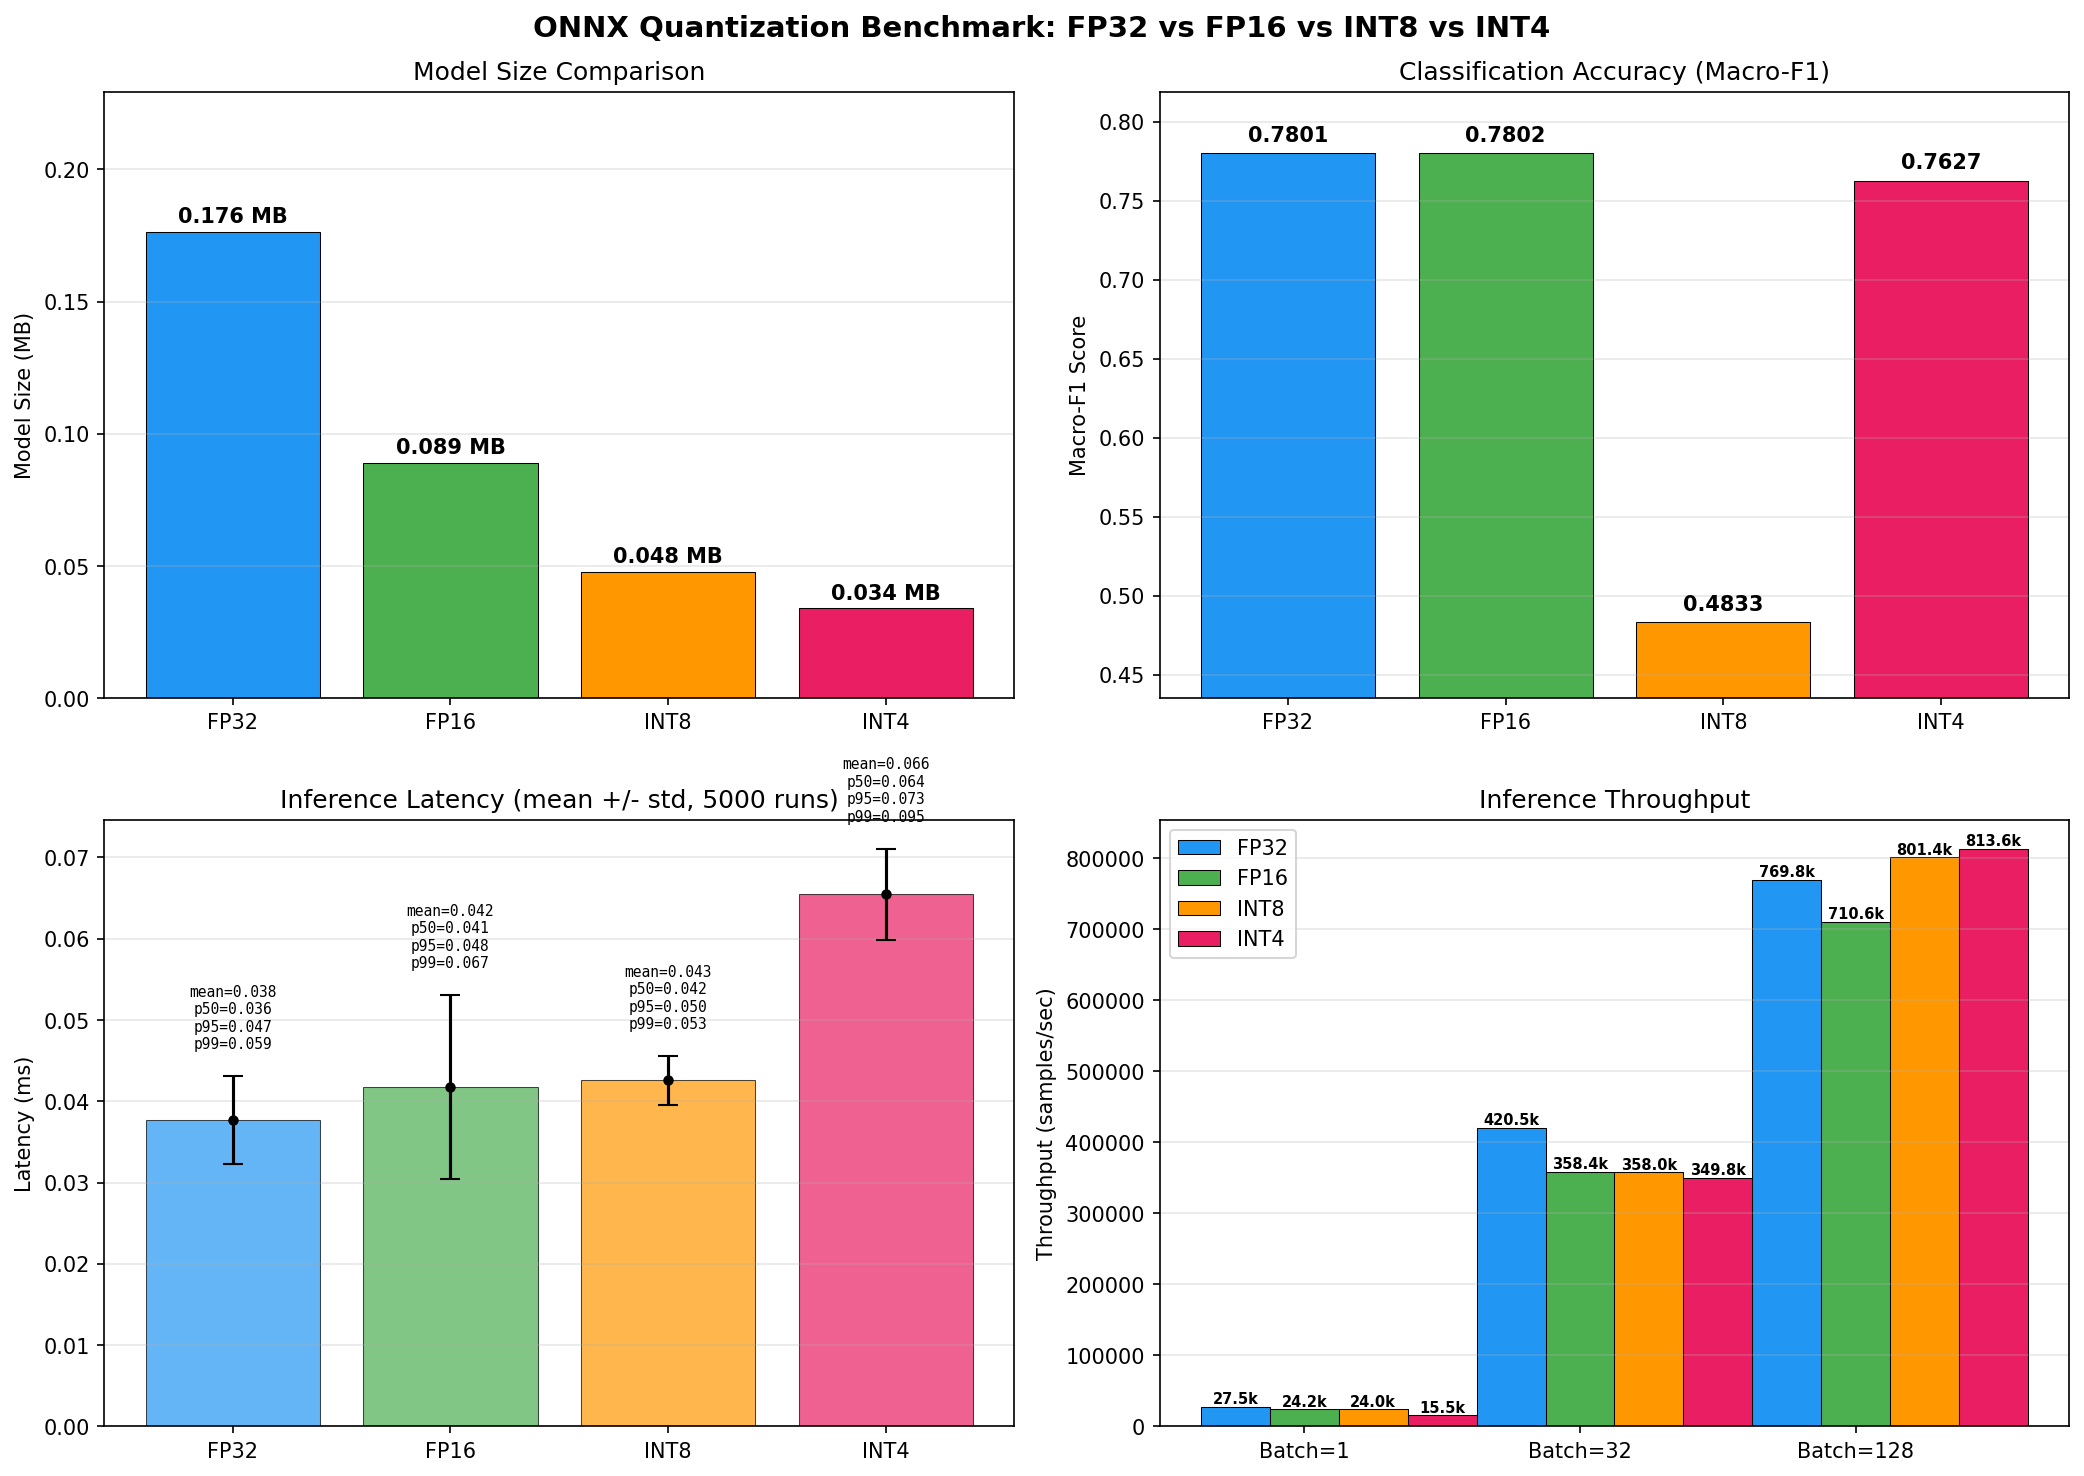
\includegraphics[width=0.85\textwidth]{figures/quantization_benchmark.png}
  \caption{Quantization benchmark across four precision levels. Top-left: model size comparison. Top-right: classification accuracy (Macro-F1), showing INT8's catastrophic degradation. Bottom-left: inference latency distribution (5,000 runs). Bottom-right: batch throughput scaling.}
  \label{fig:quantization}
\end{figure*}

\subsection{Cross-Dataset Transfer Performance}

Table~\ref{tab:crossdataset} evaluates three domain adaptation strategies for the CIC-IDS2018 $\rightarrow$ ToN-IoT transfer scenario.

\begin{table}[t]
  \centering
  \caption{Cross-Dataset Transfer: CIC-IDS2018 $\rightarrow$ NF-ToN-IoT-v2}
  \label{tab:crossdataset}
  \begin{tabular}{@{}lcc@{}}
    \toprule
    \textbf{Method} & \textbf{Binary F1} & \textbf{Multi-class F1} \\
    \midrule
    76-feat baseline (zero-filled) & 0.800 & 0.012 \\
    Source standardization & 0.800 & 0.012 \\
    Target re-standardization & 0.771 & 0.019 \\
    CORAL alignment & 0.783 & 0.005 \\
    \midrule
    NF-standardized (13 feat) & 0.766 & 0.057 \\
    \bottomrule
  \end{tabular}
\end{table}

All methods achieve reasonable binary detection (F1 $\approx$ 0.77--0.80), confirming that benign-vs-attack discrimination transfers moderately well. However, multi-class attack-type classification collapses to F1 $< 0.06$ across all methods, consistent with the findings of Pontes~\etal~\cite{pontes2021crossdataset} and Cantone~\etal~\cite{cantone2024crossdataset}. This motivates our semantic security layer: when multi-class classification is unreliable on shifted data, runtime OOD detection becomes essential for operational dependability.

\subsection{Latency Analysis}

Table~\ref{tab:latency} presents unified latency profiling across deployment modes, from raw in-memory inference to production REST API serving. Fig.~\ref{fig:latency} visualizes the latency breakdown.

\begin{table}[t]
  \centering
  \caption{Inference Latency Across Deployment Modes}
  \label{tab:latency}
  \begin{tabular}{@{}lccc@{}}
    \toprule
    \textbf{Mode} & \textbf{Mean} & \textbf{P95} & \textbf{Throughput} \\
     & \textbf{(ms)} & \textbf{(ms)} & \textbf{(flows/s)} \\
    \midrule
    \multicolumn{4}{@{}l}{\emph{Offline (in-memory, batch=1)}} \\
    \quad Plain ONNX & 0.064 & 0.066 & 27,535 \\
    \quad \sysname{} & 0.346 & 0.405 & 4,750 \\
    \quad Overhead & +0.289 & +0.339 & --- \\
    \addlinespace
    \multicolumn{4}{@{}l}{\emph{Real-time (HTTP REST streaming)}} \\
    \quad Plain REST & 4.26 & 5.81 & 235 \\
    \quad Secure REST & 5.05 & 6.06 & 198 \\
    \quad Overhead & +0.79 & +0.25 & $-$16\% \\
    \bottomrule
  \end{tabular}
\end{table}

The semantic engine adds 0.289\,ms overhead to raw ONNX inference in offline single-flow mode, but this computational cost is dominated by network and serialization I/O in REST deployment (3.26\,ms network overhead vs.\ 0.79\,ms security overhead). This demonstrates that \sysname{} is practical for real-time edge gateways.

\begin{figure*}[t]
  \centering
  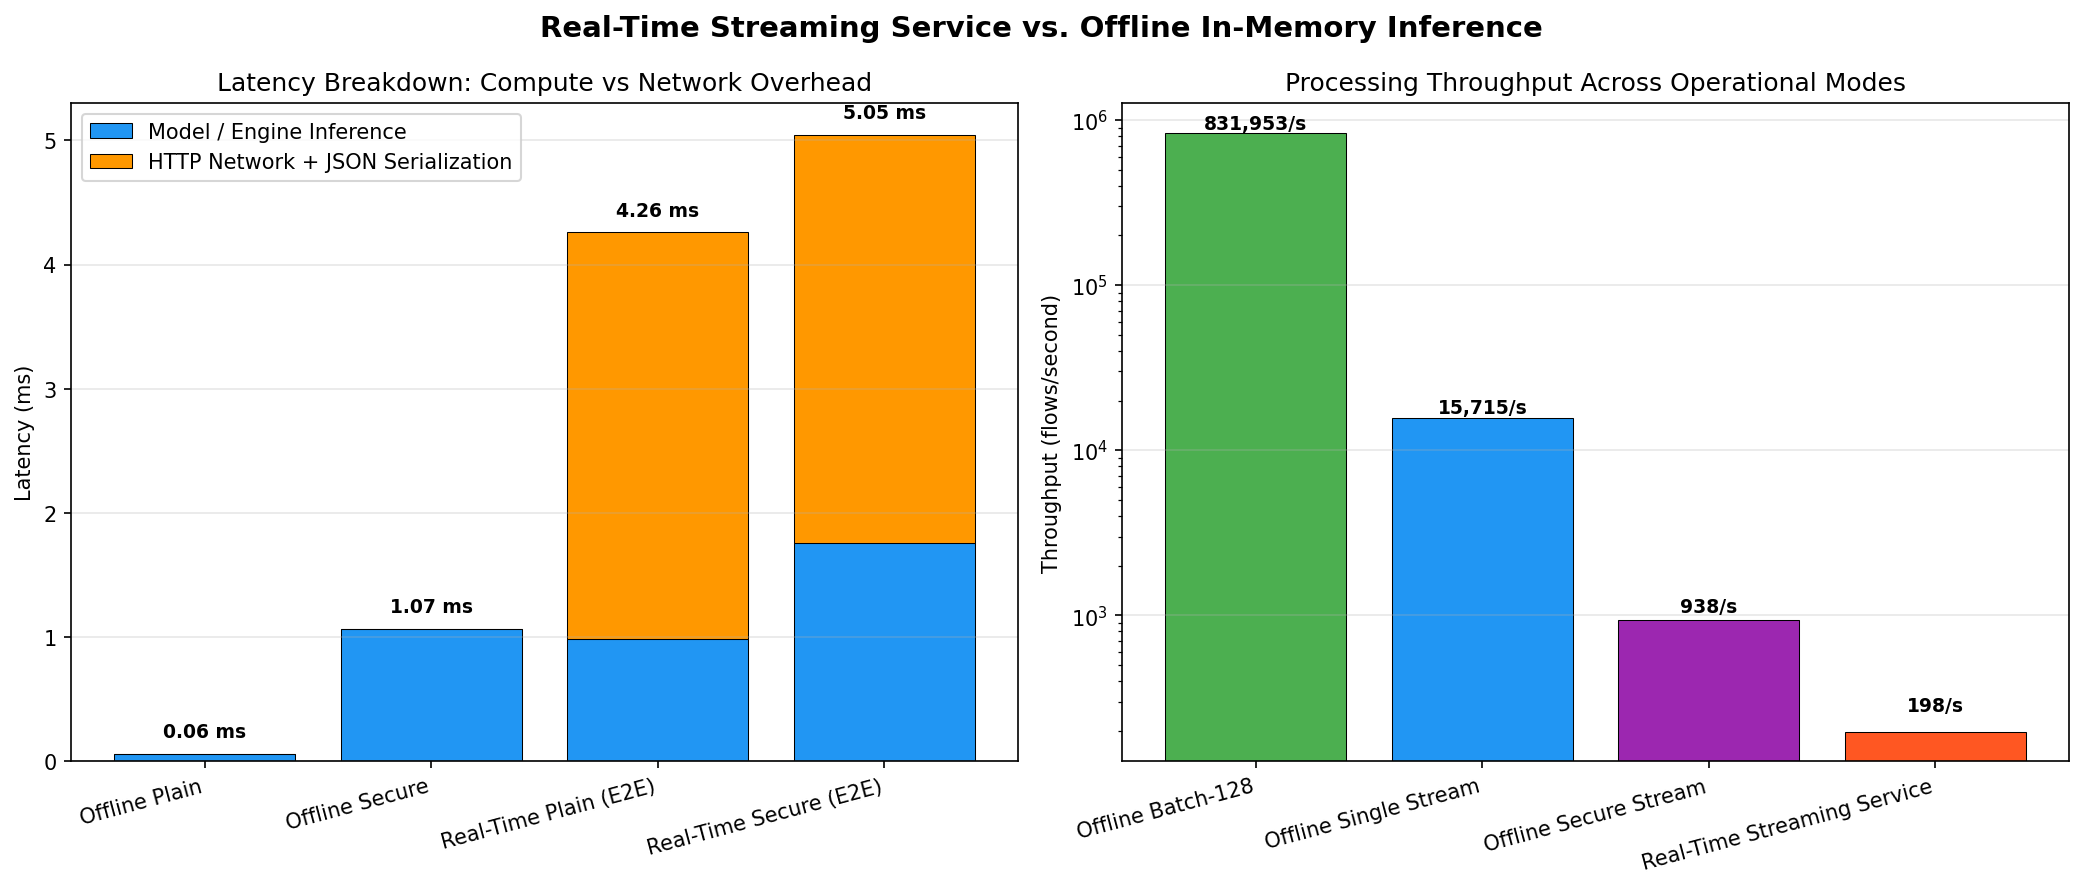
\includegraphics[width=0.85\textwidth]{figures/realtime_vs_offline.png}
  \caption{Latency breakdown: offline in-memory vs.\ real-time REST streaming. Left: per-flow latency with compute (blue) and network overhead (orange) stacked. Right: throughput across operational modes on log scale, from 831K flows/s (batch-128 offline) to 198 flows/s (secure REST streaming).}
  \label{fig:latency}
\end{figure*}


% ============================================================
% SECTION VI — DISCUSSION & LIMITATIONS
% ============================================================
\section{Discussion}
\label{sec:discussion}

\subsection{Class-Conditional Embeddings and Multi-Signal Fusion}
\label{sec:mahal_discussion}

A key architectural insight from our evaluation is the necessity of class-conditional reference modeling in multi-class network traffic. When reference metrics are computed against a single global centroid, severe class imbalance ($>80$\% benign) biases the reference coordinates toward benign traffic, causing in-distribution attack classes to appear anomalously distant while compressing out-of-distribution samples closer to the origin.

Transitioning to class-conditional distance metrics (Eqs.~\ref{eq:cosine}--\ref{eq:mahalanobis}) with $\lambda = 0.01$ covariance regularization restores geometric fidelity. Furthermore, fusing class-conditional Mahalanobis distances with output prediction confidence (Eq.~\ref{eq:drift_score}) produces a synergistic effect: the composite engine achieves AUROC = 0.966 on ToN-IoT, surpassing each component in isolation (0.959 and 0.850, respectively). This demonstrates that intermediate representations and output uncertainty provide complementary geometric signals for edge monitoring.

\subsection{Multi-Threat Coverage vs.\ Single-Metric Detectors}

While individual detectors achieve high performance on specific threat types, no single detector is universally sufficient:
\begin{itemize}[leftmargin=*]
  \item \textbf{MSP Confidence} is effective for calibrated semantic shifts (AUROC = 0.850) but blind to out-of-bounds Gaussian noise (AUROC = 0.031).
  \item \textbf{Mahalanobis Distance} excels at continuous embedding-space outliers (AUROC = 0.959) but lacks explicit schema-level protections against crafted zero-fill vectors.
  \item \textbf{Input Validator} deterministically catches 100\% of zero-fill structural failures and non-finite values before model execution.
\end{itemize}

\sysname{} unifies these monitors into a single state machine. Although alert unioning slightly increases the composite in-distribution false positive rate (13.06\% across 5 seeds compared to 5\% nominal for individual metrics), it provides robust defense across distribution drift, sensory corruption, and input tampering simultaneously.

\subsection{The INT8 Quantization Paradox}
\label{sec:int8_discussion}

Static INT8 quantization causes catastrophic accuracy degradation ($-$38\% F1) despite being a more conservative bitwidth reduction than INT4. This paradox arises from the distinction between \emph{static} and \emph{weight-only} quantization:

\textbf{Static INT8} quantizes both weights and activations to 8-bit integers, using a calibration dataset to estimate the dynamic range of intermediate activations. If the calibration data does not adequately represent the full activation range, clipping occurs: activations that fall outside the calibrated range are saturated to the minimum or maximum representable value. For the ThreatMLP architecture, the ReLU activations in layers 1--3 have long-tailed distributions that are poorly captured by the calibration step, causing widespread clipping and information loss.

\textbf{Weight-only INT4} (MatMulNBits, block size 32) quantizes only the weight matrices to 4-bit integers, while preserving FP32 precision for all activations. At inference time, weights are dequantized to FP32 before each matrix multiplication. This approach avoids the activation clipping problem entirely, at the cost of no latency improvement (dequantization adds overhead). The 80.7\% size reduction comes purely from weight compression.

This finding has practical implications: for small models where inference latency is already sub-millisecond, weight-only quantization provides the best size-accuracy trade-off, while activation quantization is only beneficial when the model is large enough that memory bandwidth dominates inference time.

\subsection{The Cross-Dataset Generalization Failure}

The central negative finding of this work---that NF-standardization does not rescue cross-dataset generalization---has two root causes that compound each other:

\begin{enumerate}[leftmargin=*]
  \item \textbf{Residual semantic mismatch:} Even after removing the 8 clearly mismatched pairs (reducing from 21 to 13 features), the remaining ``approximate match'' features introduce noise. For example, bidirectional byte counts in nProbe capture both directions of a flow, while CICFlowMeter reports forward and backward separately; concatenating them does not produce equivalent values.

  \item \textbf{Distributional shift in equivalent features:} Even for the 7 genuinely equivalent features (\eg, source port, destination port, protocol number), the statistical distributions differ fundamentally between CICFlowMeter and nProbe NetFlow processing pipelines. Different timeout configurations, flow aggregation rules, and sampling strategies produce different value distributions for the same underlying traffic.
\end{enumerate}

Neither CORAL alignment (which matches first and second moments) nor target re-standardization (which normalizes to zero mean and unit variance) meaningfully improves multi-class F1 (Table~\ref{tab:crossdataset}). This suggests that the cross-dataset generalization problem for NIDS requires \emph{training-time solutions}---multi-source training, domain-adversarial networks, or dataset-agnostic feature engineering---rather than inference-time normalization.

\subsection{Threats to Validity and Limitations}

\textbf{Architecture simplicity.} The ThreatMLP is a 4-layer MLP with ${\sim}$50K parameters, chosen specifically for edge deployment feasibility. While this limits representation capacity compared to transformers or deep residual networks, it enables sub-millisecond inference on commodity hardware. The semantic security layer is architecture-agnostic and could be applied to more complex models by re-exporting with a dual-output configuration.

\textbf{Stationary reference embeddings.} The reference centroids and covariance matrix are computed once at deployment time and do not adapt to evolving traffic patterns. Seasonal shifts, network topology changes, and new applications will gradually invalidate the reference statistics. Online centroid updating with exponential moving averages is a natural extension, though it introduces the risk of adapting to adversarial drift.

\textbf{Label taxonomy mismatch.} The ToN-IoT dataset uses attack categories (backdoor, ransomware, MITM, scanning) that do not map 1:1 to CIC-IDS2018 classes (Brute Force, DoS, Infiltration, Botnet). Approximately 23\% of ToN-IoT attack samples have no semantic equivalent in the training taxonomy, which inflates the perceived cross-dataset generalization gap.


% ============================================================
% SECTION VII — CONCLUSION
% ============================================================
\section{Conclusion}
\label{sec:conclusion}

We presented \sysname{}, a semantic security layer for ONNX-deployed NIDS classifiers that provides sub-millisecond runtime monitoring via confidence scoring, distribution drift detection, and input validation---all operating on the deployed computational graph without requiring the original training framework at inference time. Our five-seed evaluation on CSE-CIC-IDS2018 and NF-ToN-IoT-v2 demonstrates:

\begin{itemize}[leftmargin=*]
  \item \textbf{Superior OOD discrimination:} The multi-signal composite engine achieves AUROC = 0.966 for out-of-distribution traffic detection, outperforming all individual detector baselines.
  \item \textbf{Reliable threat interception:} 100\% noise detection and 100\% zero-fill rejection with only 0.29\,ms overhead on a 0.06\,ms baseline, remaining well within sub-millisecond edge budgets.
  \item \textbf{A validated negative result:} The per-field semantic schema audit reveals that 38\% of cross-dataset feature mappings measure physically different quantities. NetFlow standardization eliminates zero-filling but does not rescue multi-class cross-dataset F1, which collapses from 0.77 to 0.06.
  \item \textbf{Quantization guidance for edge deployment:} FP16 provides zero-cost 50\% compression. Static INT8 causes catastrophic accuracy loss due to activation clipping, while weight-only INT4 preserves 97.8\% of F1 with 81\% size reduction.
\end{itemize}

\textbf{Future work.} Three directions are immediately actionable: (i)~implementing online centroid adaptation with exponential moving averages to handle seasonal traffic drift without manual recalibration; (ii)~evaluating \sysname{} on hardware-specific edge platforms (Raspberry Pi 5, NVIDIA Jetson Nano) with native quantization runtime support; and (iii)~investigating domain-adversarial training for cross-extractor feature alignment.

% ============================================================
% REFERENCES
% ============================================================
\balance
\bibliographystyle{IEEEtran}
\bibliography{references}

\end{document}
